\usepackage{graphicx}
\graphicspath{{./images/}}

\begin{document}
    \thispagestyle{empty}

    \begin{center}
        Министерство науки и высшего образования Российской Федерации

        Федеральное государственно автономное образовательное учреждение высшего образования

        <<Омский государственный технический университет>>

        \vspace{1cm}
        Факультет информационных технологий и компьютерных систем

        Кафедра <<Прикладная математика и фундаметральная информатика>>

        \vspace{3cm}
        \textbf{Лабораторная работа}

        по дисциплине <<Операционные системы>>
    \end{center}
    
    \vspace{3cm}
    \begin{flushright}    
        \begin{tabular}{ r r }
            Студента & Курпенова Куата Ибраимовича \\
            \cline{2-2}
            & \tiny{фамилия, имя, отчество полностью} \\

            Курс & 2, группа ФИТ-212 \\
            \cline{2-2}
            Направление & 02.03.02 Прикладная математика \\
            \cline{2-2}
            & и фундаментальная информатика \\
            \cline{2-2}
            & \tiny{код, наименование} \\

            Руководитель & ассистент \\
            \cline{2-2}
            & \tiny{должность, ученая степень, звание} \\
            & Горшенин А. Ю. \\
            \cline{2-2}
            & \tiny{фамилия, инициалы} \\

            Выполнил & \\
            \cline{2-2}
            & \tiny{дата, подпись студента(ки)} \\
        \end{tabular}
    \end{flushright}
    
    \vspace*{\fill}
    \begin{center}
        Омск 2022
    \end{center}

    \newpage

    \section*{Задание 1}

    Разработать в Linux программу, которая получает хэндлы стандартного ввода и вывода, выводит числовые с комментариями значения этих хэндлов, затем, используя стандартный ввод системными функциями небуферизованного ввода-вывода ReadFile или WriteFile, делает приглашение для ввода, вводит любой текст и выводит его с предуведомлением, что он предварительно введен в программу, обеспечивая в этой системе вывод приглашения на ввод данных со стандартного ввода только в случае использовании ввода с консоли, при переадресации этого ввода на входной файл приглашение отображаться не должно. При переадресации стандартного вывода в файл отображение приглашения в случае ввода с консоли должно принудительно появляться на экране, а не в файле, на который переадресуется вывод. Числовые значения хэндлов стандартных ввода и вывода в этом варианте выводить не нужно.

    \subsection*{Решение}

    \begin{figure}[H]
        \centering
        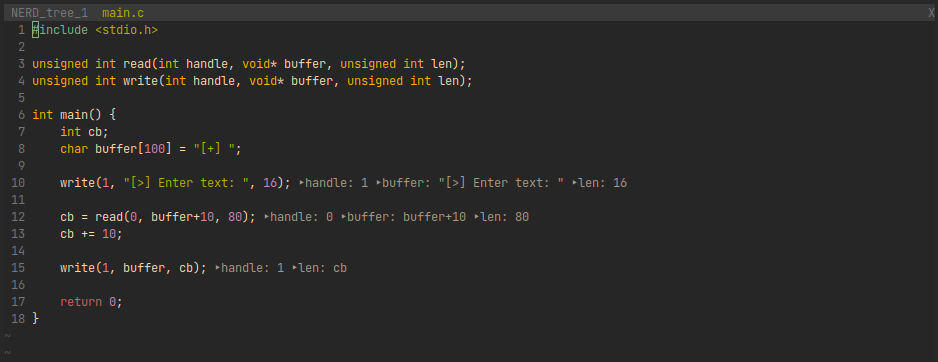
\includegraphics[width=\textwidth]{images/lab1/solution.png}
        \caption{Код программы main.c}
    \end{figure}

    \begin{figure}[H]
        \centering
        \includegraphics[width=\textwidth]{images/lab1/result.png}
        \caption{Вывод программы main.c}
    \end{figure}

    \newpage

    \section*{Задание 2}

    Результат выполнения лабораторной работы должен состоять из двух программ для Linux. Первая программа должна создавать текстовый файл, вводя данные со стандартного ввода. (Более детально: открывает файл для записи, читает текст со стандартного ввода и выводит этот прочитанный текст в файл.) Вторая программа открывает тот же файл (созданный перед этим другой программой) для чтения и хэндл, полученный при этом открытии, запоминает в 1-й переменной для хэндла. Используя этот хэндл, далее с помощью функции dup() получается новое значение хэндла для доступа к тому же файлу (2-й хэндл). Еще раз открывается тот же файл, запоминая 3-е значение хэндла. С помощью первого хэндла программа позиционирует чтение для 10-й позиции файла от начала этого файла. Далее программа должна выводить числовые значения всех трех хэндлов на экран. Используя по очереди все 3 хэндла, из файла читаются по 7 символов и тут же эти три прочитанных текста выводятся на экран, каждая в своей строке. Результаты вывода объяснить.

    \subsection*{Решение}

    \begin{figure}[H]
        \centering
        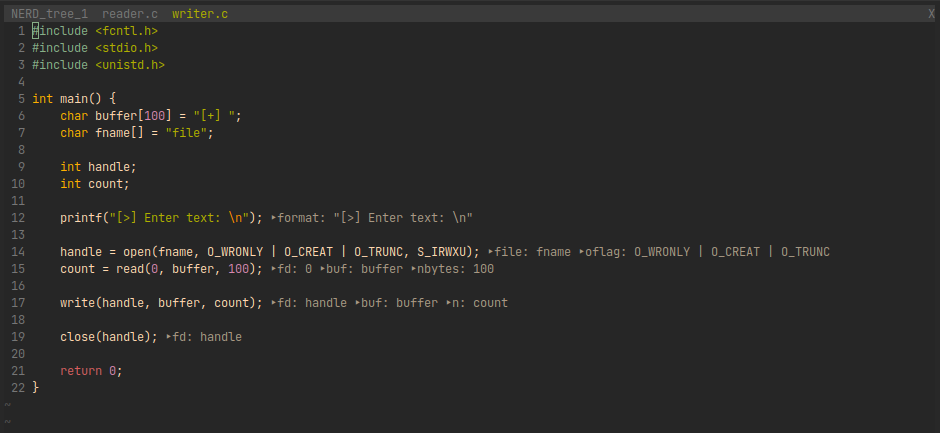
\includegraphics[width=\textwidth]{images/lab2/writer.png}
        \caption{Код программы writer.c}
    \end{figure}

    \begin{figure}[H]
        \centering
        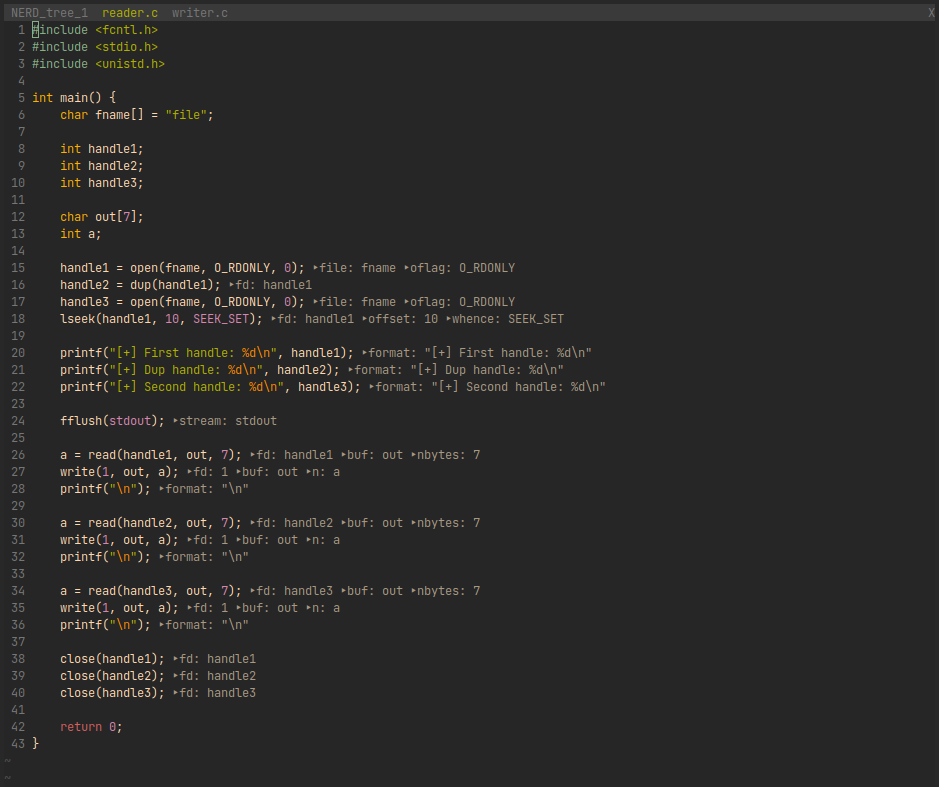
\includegraphics[width=\textwidth]{images/lab2/reader.png}
        \caption{Код программы reader.c}
    \end{figure}

    \begin{figure}[H]
        \centering
        \includegraphics[width=\textwidth]{images/lab2/result.png}
        \caption{Результат работы программ writer.c и reader.c}
    \end{figure}

    \newpage

    \section*{Задание 7}

    Разработать программу с тремя дополнительными нитями (threads) относительно главной нити. Каждая из нитей должна использовать общие для всех нитей данные, представленные массивом символов, в которых записаны 20 первых букв латинского алфавита. Каждая из этих нитей на своем k-м шаге выводит со своей случайной задержкой на место «своего» столбца экрана k-ю букву из указанного массива латинских букв, причем с числом повторений, равному условному номеру нити, умноженному на два. Каждая из используемых нитей должен осуществлять вывод своим цветом, отличным от остальных нитей. На 6-м шаге главная нить делает попытку отмены первой из дополнительных нитей, а на 11-м делает попытку отмены третьей из дополнительных нитей. Первая и третья дополнительная нити в начале своей работы запрещают свою отмену. Третья нить на 13 шаге разрешает отмену, но в отложенном режиме. Точку отмены эта нить устанавливает между 16 и 17-м шагом своей работы. Все управляющие указания должны отображаться сообщениями без прокрутки экрана (в фиксированные позиции экрана).

    \subsection*{Решение}

    \begin{figure}[H]
        \centering
        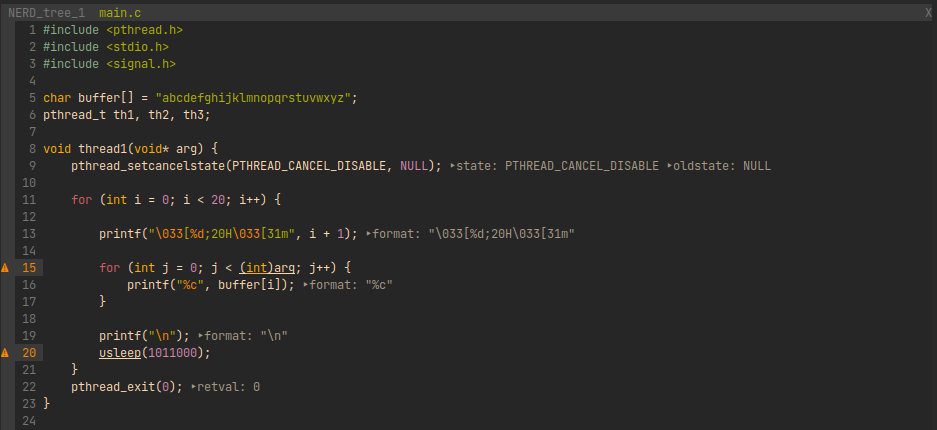
\includegraphics[width=\textwidth]{images/lab7/thread1.png}
        \caption{Код метода thread1}
    \end{figure}

    \begin{figure}[H]
        \centering
        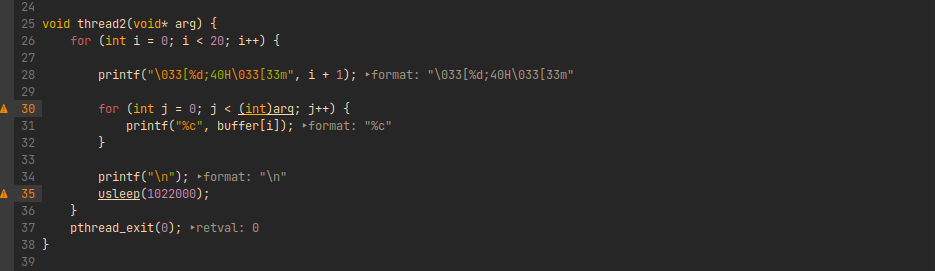
\includegraphics[width=\textwidth]{images/lab7/thread2.png}
        \caption{Код метода thread2}
    \end{figure}

    \begin{figure}[H]
        \centering
        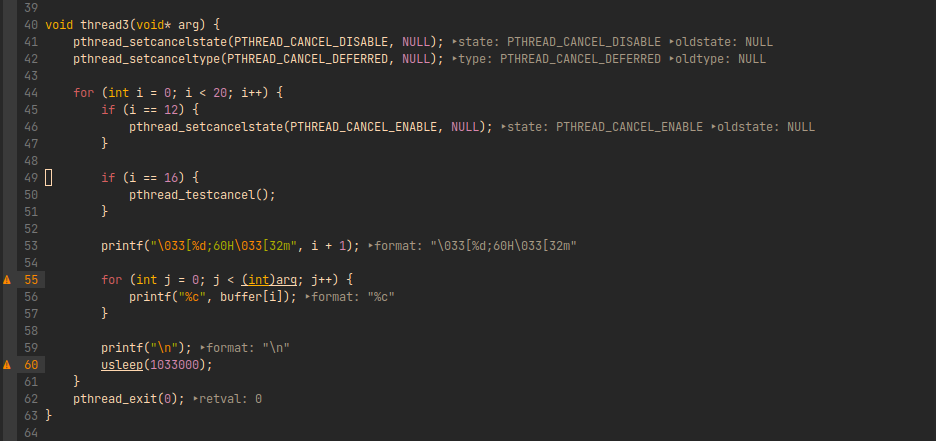
\includegraphics[width=\textwidth]{images/lab7/thread3.png}
        \caption{Код метода thread3}
    \end{figure}

    \begin{figure}[H]
        \centering
        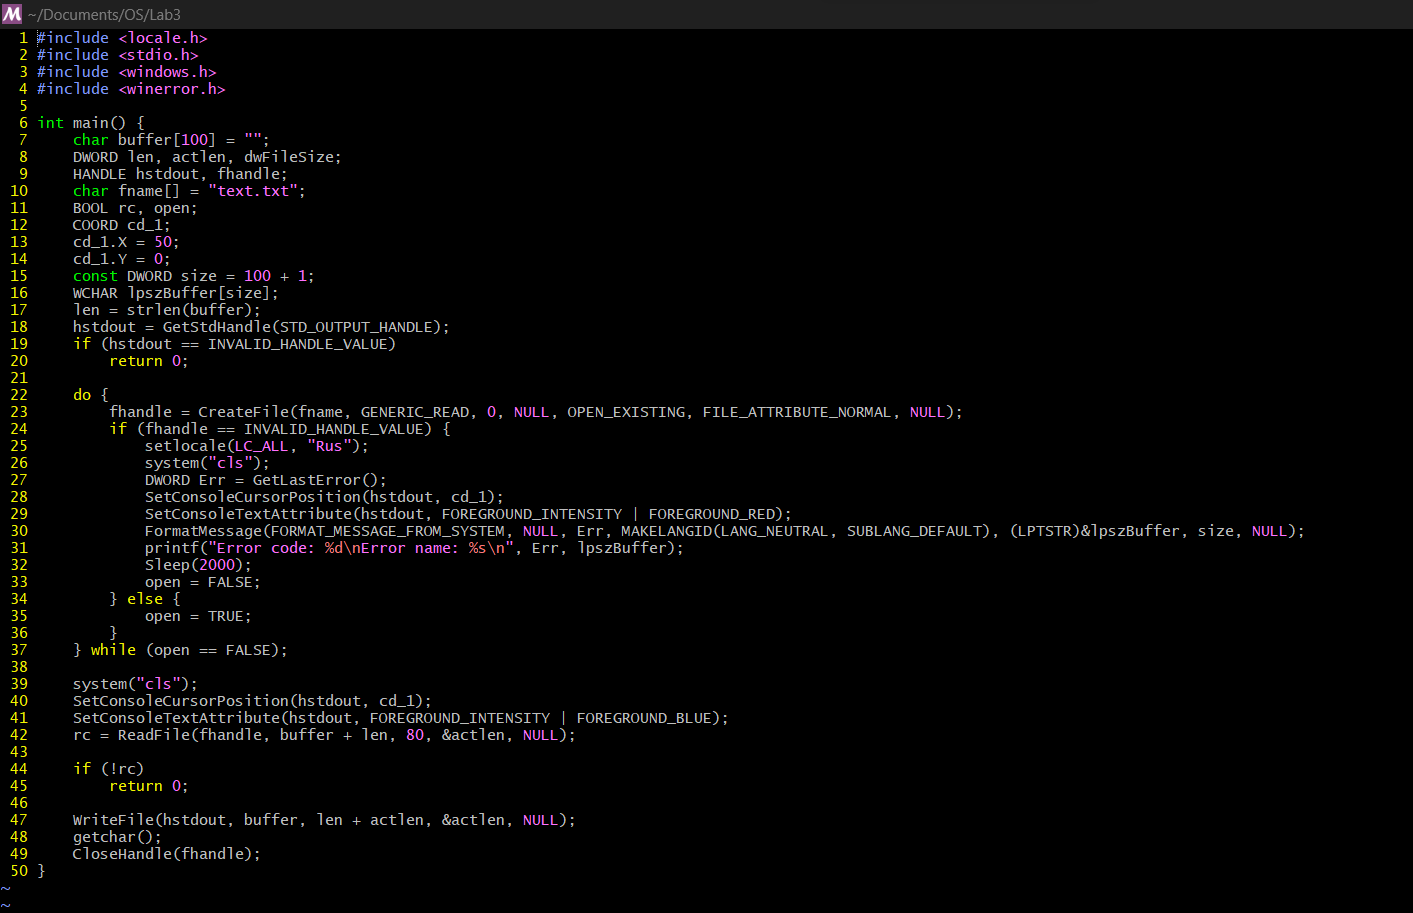
\includegraphics[width=\textwidth]{images/lab7/main.png}
        \caption{Код метода main}
    \end{figure}

    \begin{figure}[H]
        \centering
        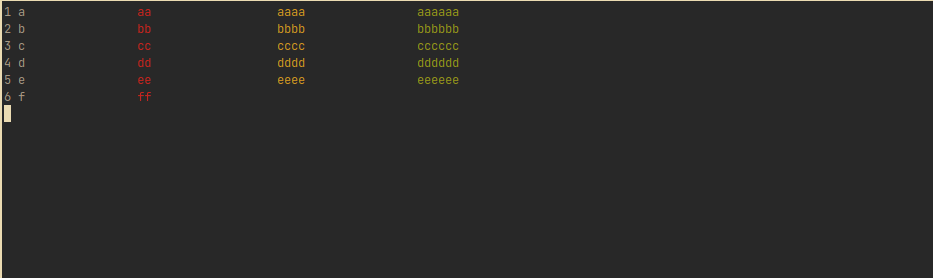
\includegraphics[width=\textwidth]{images/lab7/result1.png}
        \caption{Результат работы программы в момент работы первого потока}
    \end{figure}

    \begin{figure}[H]
        \centering
        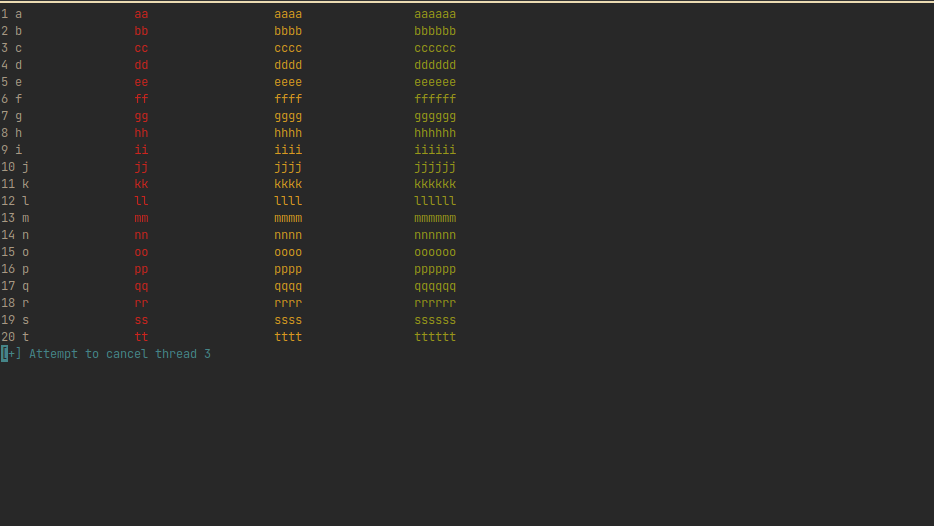
\includegraphics[width=\textwidth]{images/lab7/result2.png}
        \caption{Результат работы программы в момент работы третьего потока}
    \end{figure}

    \newpage
    
\end{document}
